\documentclass[11pt]{article}
\usepackage[utf8]{inputenc}
\usepackage[margin=0.8in]{geometry}
\usepackage{amsfonts, amsmath}
\usepackage{tikz}
\usepackage[nobreak=false]{mdframed}
\usepackage{pgf}
\usepackage{enumitem}
\usepackage{mathtools}
\usepackage{bbm}
\usepackage{graphicx}
\usepackage{url}
\usepackage{enumitem}
\usepackage{amsthm,amssymb}
\usepackage{float}
\usepackage{minted}
\setlength\parindent{0pt}
\newcommand{\solution}{\subsection*{Solution:}}
\DeclareMathOperator*{\argmax}{arg\!max}
\DeclareMathOperator*{\argmin}{arg\!min}
\DeclareMathOperator*{\trace}{trace}
\graphicspath{{./figs/}}

\begin{document}

\title{EE127 Homework 4}
\author{Vighnesh Iyer}
\date{\today}
\maketitle

\subsection*{Exercise 1 (Quadratic inequalities)}

Consider the set defined by the following inequalities
\[
\left( x_1 \ge x_2 - 1 \mbox{ and } x_2 \ge 0 \right) \mbox{ or }
\left( x_1 \le x_2 - 1  \mbox{ and } x_2 \le 0 \right).
\]
\begin{enumerate}
\item
Draw the set.  Is it convex?
\item
Show that it can be described as a single quadratic inequality of the form $q(x) = x^T A x + 2 b^T x + c \leq 0$, for matrix $A=A^T  \in \mathbb{R}^{2,2}$, $b \in \mathbb{R}^{2}$ and $c \in \mathbb{R}$ which you will determine.
\item What is the convex hull of this set?
\end{enumerate}

\begin{solution}
\begin{enumerate}
    \item
    \begin{figure}[H]
        \centerline{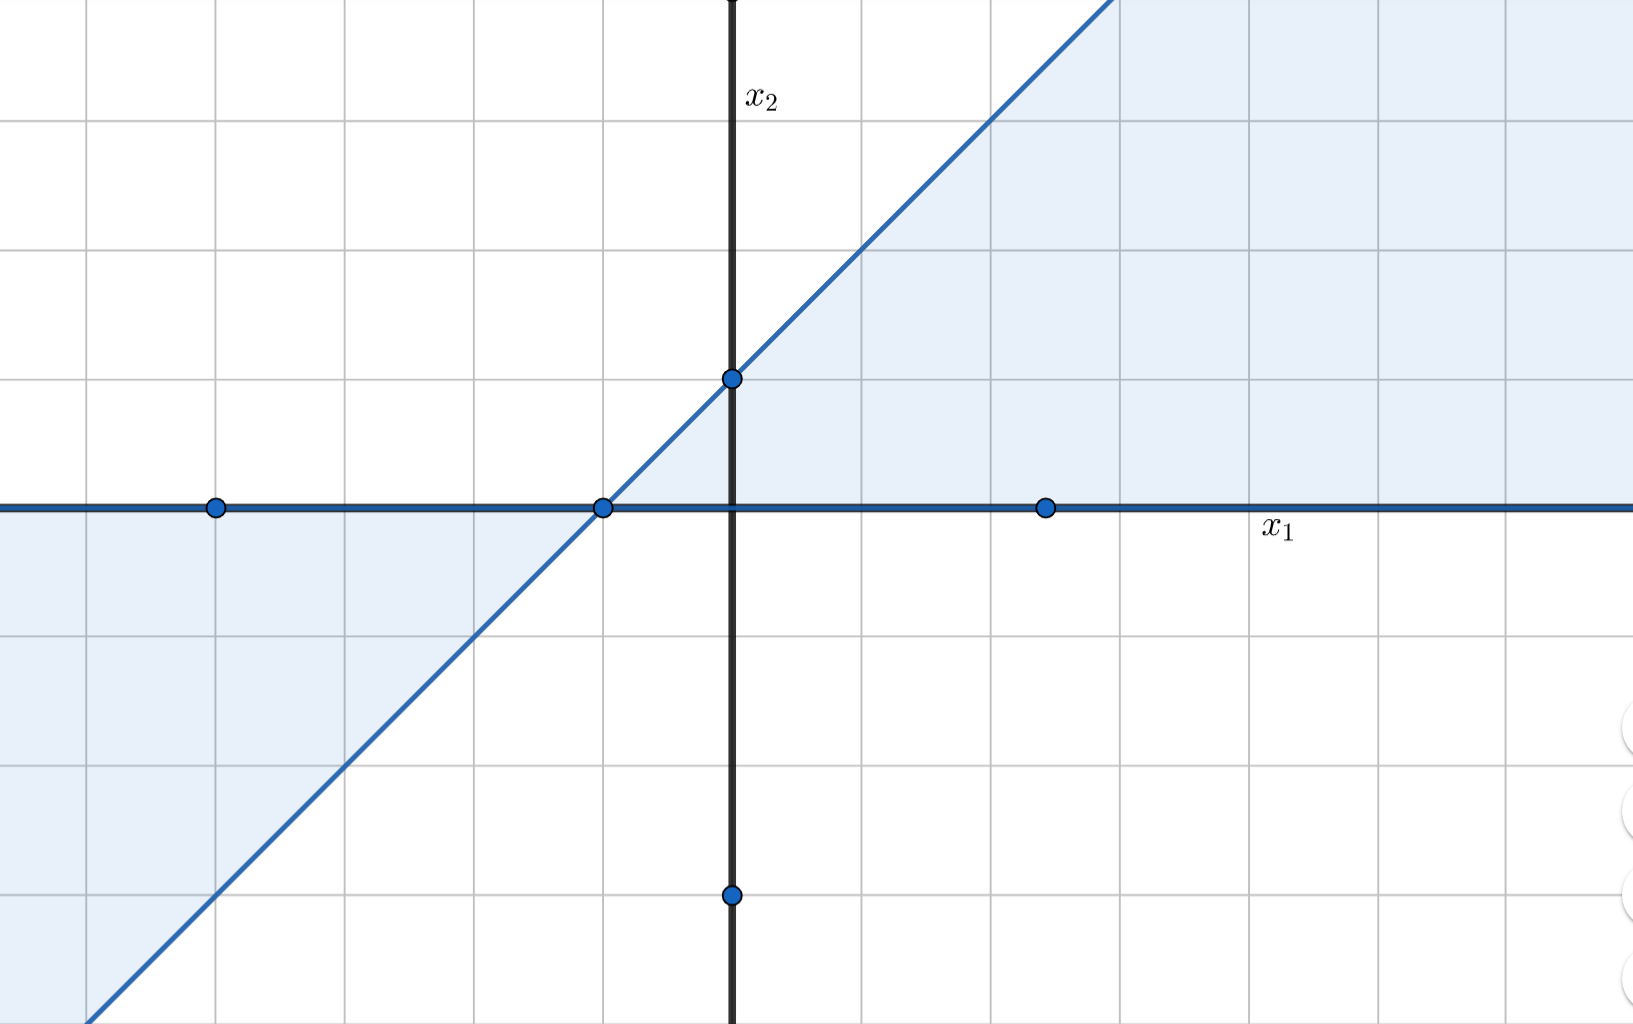
\includegraphics[width=0.6\textwidth]{problem1_set.png}}
    \end{figure}
    This set is not convex because we can choose a pair of points in the set for which a line between these points contains points not in the set. As an example choose (-2, -1) and (1, 0). The line between these points contains points not in the set.

    \item Start with an observation about $ab \geq 0$ and apply it to this problem:
    \begin{align*}
        ab \geq 0 &\rightarrow (a \geq 0 \cap b \geq 0) \cup (a \leq 0 \cap b \leq 0) \\
        &(x_1 - x_2 + 1 \geq 0 \cap x_2 \geq 0) \cup (x_1 - x_2 + 1 \leq 0 \cap x_2 \leq 0) \\
        a &= x_1 - x_2 + 1 \\
        b &= x_2 \\
        (x_1 - x_2 + 1) x_2 &\geq 0 \\
        x_1 x_2 - x_2^2 + x_2 &\geq 0 \\
        x_2^2 - x_1 x_2 - x_2 &\leq 0
    \end{align*}
    Translating into quadratic matrices:
    \begin{align*}
        A &= \begin{bmatrix} 0 & -\frac{1}{2} \\ -\frac{1}{2} & 1 \end{bmatrix} \\
        b &= \begin{bmatrix} 0 \\ -\frac{1}{2} \end{bmatrix} \\
        c &= 0
    \end{align*}

\item The convex hull of a set is the minimal convex set in $\mathbb{R}^2$ that contains the set. In this case that is the entire $\mathbb{R}^2$ space. Looking at the set when $x_2 \leq 0$ one can draw an infinite set of lines from the points on the corners of the set. These lines cover the entire space $x_2 \leq 0$ that isn't covered by the existing set. A similar argument can be made for $x_2 \geq 0$ and thus the entire $\mathbb{R}^2$ space is the convex hull.
\end{enumerate}
\end{solution}

\newpage
\subsection*{Exercise 2 (Formulating problems as LPs or QPs)}

Formulate the problem
\[
p_j^* \doteq \min_x \: f_j(x),
\]
for different functions $f_j$, $j=1,\ldots,4$, as QPs or LPs, or, if you cannot, explain why.
In our formulations, we always use $x \in \mathbb{R}^{n}$ as the variable, and assume that $A \in \mathbb{R}^{m,n}$, $y \in \mathbb{R}^{m}$. If you obtain an LP or QP formulation, make sure to put the problem in standard form, stating precisely what the variables, objective, and constraints are.
\begin{center}
\begin{tabular}{rcl}
$f_1(x)$  &=& $\|Ax-y\|_\infty +\|x\|_1$ \\
$f_2(x)$  &=& $\|Ax-y\|_2^2 + \|x\|_1$ \\
$f_3(x)$  &=& $\|Ax-y\|_2^2 - \|x\|_1$ \\
$f_4(x)$  &=& $\|Ax-y\|_2^2 + \|x\|_1^2$
\end{tabular}
\end{center}

\begin{solution}
\begin{enumerate}
    \item \begin{align*}
        \min_{x} f_1(x) &= \min_{x} \|Ax-y\|_\infty + \|x\|_1 \\
        &= \min_{x,t} t + \|x\|_1 : \|Ax-y\|_\infty \leq t \\
        &= \min_{x,t,u} t + \mathbbm{1}_n u : |x_i| \leq u_i \quad \forall i = 1, \dots, n
    \end{align*}
    In total:
    \begin{align*}
        &\min_{x,t,u} t + \mathbbm{1}_n u \\
        &(|A x - y|)_i \leq t \quad \forall i = 1, \dots, m \\
        &|x_i| \leq u_i \quad \forall i = 1, \dots, n
    \end{align*}
    The absolute value inequality constraints can be written as two one-sided constraints. This is an LP.

    \item We can expand the squared 2-norm term to get a QP and can express the 1-norm term in the same way as the previous problem.
    \begin{align*}
        \min_{x} f_2(x) &= \min_{x,t} x^T A^T A x - 2 x^T A^T y + y^T y + \mathbbm{1}_n t \\
        &|x_i| \leq t_i \quad \forall i = 1, \dots, n
    \end{align*}

    \item The objective isn't convex. Take the case where $n = 1, A = 1, y = 0$ then $f_3(x) = x^2 - |x|$. Looking at the graph:
    \begin{figure}[H]
        \centerline{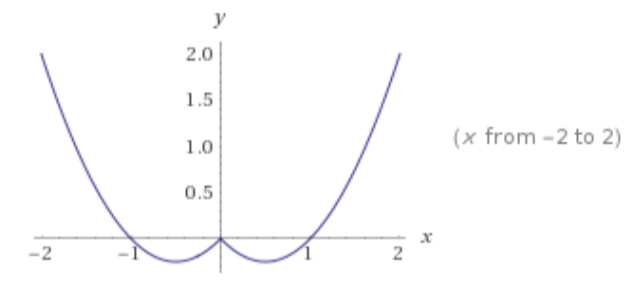
\includegraphics[width=0.3\textwidth]{problem2_plot.png}}
    \end{figure}
    We can see the epigraph isn't a convex set because a line segment can be drawn from $(-0.1, f_3(-0.1))$ to $(0.1, f_3(0.1))$ which crosses points not in the set.

    \item \begin{align*}
        \min_x f_4(x) &= \min_x \|Ax - y\|_2^2 + (\sum_{i=1}^n |x_i|)^2 \\
        \text{by C-S } &\leq \min_x \|Ax - y\|_2^2 + n \sum_{i=1}^n |x_i|^2 \\
        &= \min_x \|Ax-y\|_2^2 + n (x_1^2 + \dots + x_n^2) \\
        &= \min_{x} x^T A^T A x - 2 x^T A^T y + y^T y + n (x_1^2 + \dots + x_n^2)
    \end{align*}

    This is an unconstrained QP. To find the real solution, plug in $\argmin_x$ to the original function.
\end{enumerate}
\end{solution}

\newpage
\subsection*{Exercise 3 (Regularized least-squares problem with low-rank data)}

Consider the problem
\[
p^* \doteq \min_{x} \: \|Ax - y\|_2^2+ \lambda \|x\|_2^2
\]
where $A \in \mathbb{R}^{m,n}$, $y \in \mathbb{R}^{m}$ and the penalty parameter $\lambda \ge 0$ are given. In this exercise, we show that if $A$ is low-rank, and a low-rank decomposition is known, then we can exploit that structure to greatly reduce the computational burden involved.

\begin{enumerate}
    \item Assume that $A$ has rank $r << \min(n,m)$, and that a low-rank decomposition of $A$ is of the form $A = LR^T$ is known, with $L \in \mathbb{R}^{m,r}$, $R \in \mathbb{R}^{n,r}$ both full rank. Explain how to reduce the problem to one with $r$ variables only.

    \item Discuss the complexity of the method and compare it to that of a ``direct'' approach where the low-rank structure is ignored.

    \item In the notebook \verb+lpqp_low_rank_ls.ipynb+, we have generated some random data for $r=10, m=1000, n=1000$. Implement the direct approach and compare it with the low-rank approach.

    \item We investigate how this approach can be used even when the data is full-rank. In particular, we generated a full-rank data matrix $A$ for $m=300, n=300$ in the second part of the notebook \verb+lpqp_low_rank_ls.ipynb+ but for which most of the variance is explained in the first $\hat{r}$ eigenvalues. In that particular case, we provide you with code that approximates your matrix $A$ with $\hat{A}$ of rank $r$ for all $r$, solves the low-rank problem based on your previous code, and plots the error $p^*$ as a function of $r$. Use this graph to make a guess about $\hat{r}$ and interpret.
\end{enumerate}

\begin{solution}
\end{solution}

\newpage
\subsection*{Exercise 4 (A Boolean problem of maximal margin)}

We have to decide which items to sell among of a collection of $n$ items, with given selling prices $s_i>0$, $i=1,\ldots,n$. Selling implies a transaction cost $c_i>0$ for each item $i$; the total transaction cost is the sum of these costs, plus a fixed amount $d>0$ (say, $d=1$). We are interested in the following decision problem: which items need to be sold, in order to maximize the margin (revenue-to-cost ratio). \textit{Assume a transaction will occur for all items we choose to sell.}

\begin{enumerate}
    \item Show that the problem can be formalized as
    \[
    p^* \doteq \max_{x \in \{0,1\}^n} \: f(x), \;\; f(x) \doteq \frac{s^T x}{1+c^T x} .
    \]

    \item Show that the problem admits a one-dimensional formulation:
    \[
    p^* = \min_{t \ge 0} \: t ~:~ t  \ge \mathbf{1}^T (s-tc)_+.
    \]
    Here $z_+$, for a vector $z \in \mathbb{R}^{n}$, denotes the vector with components $\max(0,z_i)$, $i=1,\ldots,n$. {\em Hint:} for given $t \ge 0$, express the condition $f(x) \le t$ for every $x \in \{0,1\}^n$ in simple terms.

    \item Let us assume the inequality constraint $t \ge \mathbf{1}^T (s-ct)_+$ is active at optimum. How can you recover an optimal solution $x^*$ from an optimal value $t^*$ for the above problem?
\end{enumerate}

\begin{solution}
\begin{enumerate}
    \item Let $x \in \{0,1\}^n$ be a vector such that $x_i = 1$ means we are selling item $i$ and $x_i = 0$ if we aren't selling item $i$.

    Then revenue $R = s^T x$ and cost $C = c^T x + d$ where $d = 1$. Thus we can formalize this problem as the optimization:
    \begin{align*}
        p^* = \max_{x \in \{0,1\}^n} f(x), \quad f(x) = \frac{s^T x}{c^T x + 1}
    \end{align*}

    \item Note:
    \begin{align*}
        \max_x f_0(x) &= \min_{x,t} t \quad : \quad f_0(x) \leq t \\
        t^* &= \max_x f_0(x)
    \end{align*}

    For any $t \geq 0$ we can write $f(x) \leq t$ as:
    \begin{align*}
        \frac{s^T x}{c^T + 1} &\leq t \\
        t c^T x + t &\geq s^T x \\
        t &\geq s^Tx - t c^T x \geq 0 \\
        t &\geq (s_1 - t c_1)x_1 + \dots + (s_n - t c_n)x_n \geq 0 \\
        t &\geq \mathbf{1}_n (s-tc)_{+}
    \end{align*}

    Note that we can set $x_i$ to 0 if $s_i - t c_i$ is negative to make sure $t \geq 0$ is satisfied.

    Then, putting this in standard form:
    \begin{align*}
        p^* = \min_{t \geq 0} t \quad : \quad t \geq \mathbf{1}^T (s - tc)_{+}
    \end{align*}

    \item At optimum $t^* = (s_1 - c_1 t^*)x_1 + \dots + (s_n - c_n t^*)x_n$. To recover $x_i$, just set it to 1 if $(s_i - c_i t^*)$ is positive else set it to zero.
\end{enumerate}
\end{solution}

\newpage
\subsection*{Exercise 5 (Robust production plans)}

Recall the drug production problem discussed in lectures 10 (slide 22) and 13. A company produces two kinds of drugs, DrugI and DrugII, containing a specific active agent A, which is extracted from raw materials purchased on the market. There are two kinds of raw materials, RawI and RawII, which can be used as sources of the active agent.  The related production, cost and resource data are given next.  The goal is to find the production plan which maximizes the profit of the company. \\ \\
Let $x_{\text{rmDrugI}}$, $x_{\text{rmDrugII}}$ denote the amounts (in 1000 of packs) of Drug I and II produced, while $x_{\text{rmRawI}}$, $x_{\text{rmRawII}}$ denote the amounts (in kg) of raw materials to be purchased. We seek to find the production and raw material amounts that maximize profit (revenue minus cost). Furthermore, we are subject to constraints on the balance of the active agent, storage, manpower, equipment, and budget, and constrain all variables to be non-negative. \\ \\

Putting this together, we get the LP:
\begin{align*}
    \min_{x} c^T x \; \; : Ax \leq b, \; x \geq 0.
\end{align*}
where $x= (x_{\text{RawI}},x_{\text{RawII}},x_{\text{DrugI}},x_{\text{DrugII}})$. For details on how this optimization problem is formulated, please see slide 22 in lecture 10.

We now assume that the vector $c$, which represents cost minus revenue, is subject to scenario uncertainty. Precisely, $c$ is only known to belong to a given set of the form
\[
{\cal C} = \left\{ c^{(k)} = \hat{c} + \rho \delta c^{(k)}, \;\; k=1,\ldots,K \right\},
\]
where $\hat{c} \in \mathbb{R}^{4}$ is the nominal value, $\delta c^{(k)}$ is the $k$-th scenario and $\rho \geq 0$ is a measure of uncertainty. To any given candidate solution $x \in \mathbb{R}^{4}$, we define the worst-case cost as
\[
p^{\rm wc}(x) := \max_{c \in {\cal C}} \: c^Tx.
\]
We have loaded the data for this problem in the notebook {\tt drug\_prod.ipynb}.
\begin{enumerate}
\item Solve for the nominal problem's solution $x^{\rm nom}$, in which $c = \hat{c}$, and compute the profit. Compute the worst-case profit of this plan.

\item Derive the robust counterpart of the problem, based on optimizing the worst-case cost. Compare the robust solution to the nominal one, in terms of nominal cost and in terms of worst-case cost, and comment.

\item Plot the elements of the robust solution as the uncertainty level $\rho$ grows. What is the smallest value of $\rho$ for which the robust solution is zero?

\end{enumerate}

\begin{solution}
\begin{enumerate}
    \item
        \begin{minted}{python}
def solve_nominal(A, b, c_hat):
    x_nom = cp.Variable(4)
    objective = cp.Minimize(cp.sum(c_hat * x_nom))
    constraints = [
        A * x_nom <= b,
        x_nom >= 0
    ]
    prob = cp.Problem(objective, constraints)
    result = prob.solve()
    return x_nom.value, result
        \end{minted}
        \begin{minted}{python}
def worst_cost(x, c_hat, rho, deltaC):
    costs = [np.dot(np.add(c_hat, np.multiply(rho, ck)), x) for ck in deltaC]
    return np.max(costs)
        \end{minted}
        \begin{minted}{python}
x_nom, cost_nom = solve_nominal(A, b, c_hat)
print('x_nom:\n{}'.format(x_nom))
print('profit_nom: {}'.format(-1. * cost_nom))
print('worst_profit: {}'.format(-1. * worst_cost(x_nom, c_hat, rho, deltaC)))
        \end{minted}
        \begin{minted}{text}
x_nom:
[4.95900359e-06 4.38788940e+02 1.75515577e+01 5.85913325e-10]
profit_nom: 8819.657742458643
worst_profit: 1515.528520317108
        \end{minted}

    \item We are solving:
    \begin{align*}
        \min_x p^{wc}(x) = \min_x \max_{c \in C} c^T x \quad : \quad Ax \leq b, x \geq 0
    \end{align*}
    To solve this, introduce a slack variable to pull the $\max$ function into the constraints, and then enumerate the $max$ function over all $c^{(k)}$.
    \begin{align*}
        \min_{x, t} t \quad : \quad Ax \leq b, x \geq 0, t &\geq \max_{c \in C} c^T x \\
        t &\geq c^{(i)T} x \quad \forall i = 1, \dots, K
    \end{align*}
    \begin{minted}{python}
def solve_robust(A, b, c_hat, rho, deltaC):
    x_rob = cp.Variable(4)
    t = cp.Variable(1)
    objective = cp.Minimize(t)
    constraints = [
        A * x_rob <= b,
        x_rob >= 0,
    ]
    rob_constraints = [t >= cp.sum((c_hat + np.multiply(rho, ck)) * x_rob) for ck in deltaC]
    all_constraints = constraints + rob_constraints
    prob = cp.Problem(objective, all_constraints)
    result = prob.solve()
    return x_rob.value, result
    \end{minted}
    \begin{minted}{python}
x_rob, cost_rob = solve_robust(A, b, c_hat, rho, deltaC)
print('x_rob:\n{}'.format(x_rob))
print('profit_rob: {}'.format(-1. * cost_rob))
print('worst_profit: {}'.format(-1. * worst_cost(x_rob, c_hat, rho, deltaC)))
    \end{minted}
    \begin{minted}{python}
x_rob:
[8.77192982e+02 4.48255474e-08 1.75438596e+01 4.02905624e-10]
profit_rob: 5689.9470812993395
worst_profit: 5689.947081802748
    \end{minted}
    The robust solution optimizes for maximizing the worst case profit, so the worst case profit is equal to the solution itself. The robust optimal $x_{rob}$ yields a smaller nominal cost than the nominal $x_{nom}$.

    \item
    The smallest value of $\rho$ for which the robust solution is 0 is around 0.085.
    \begin{figure}[H]
        \centerline{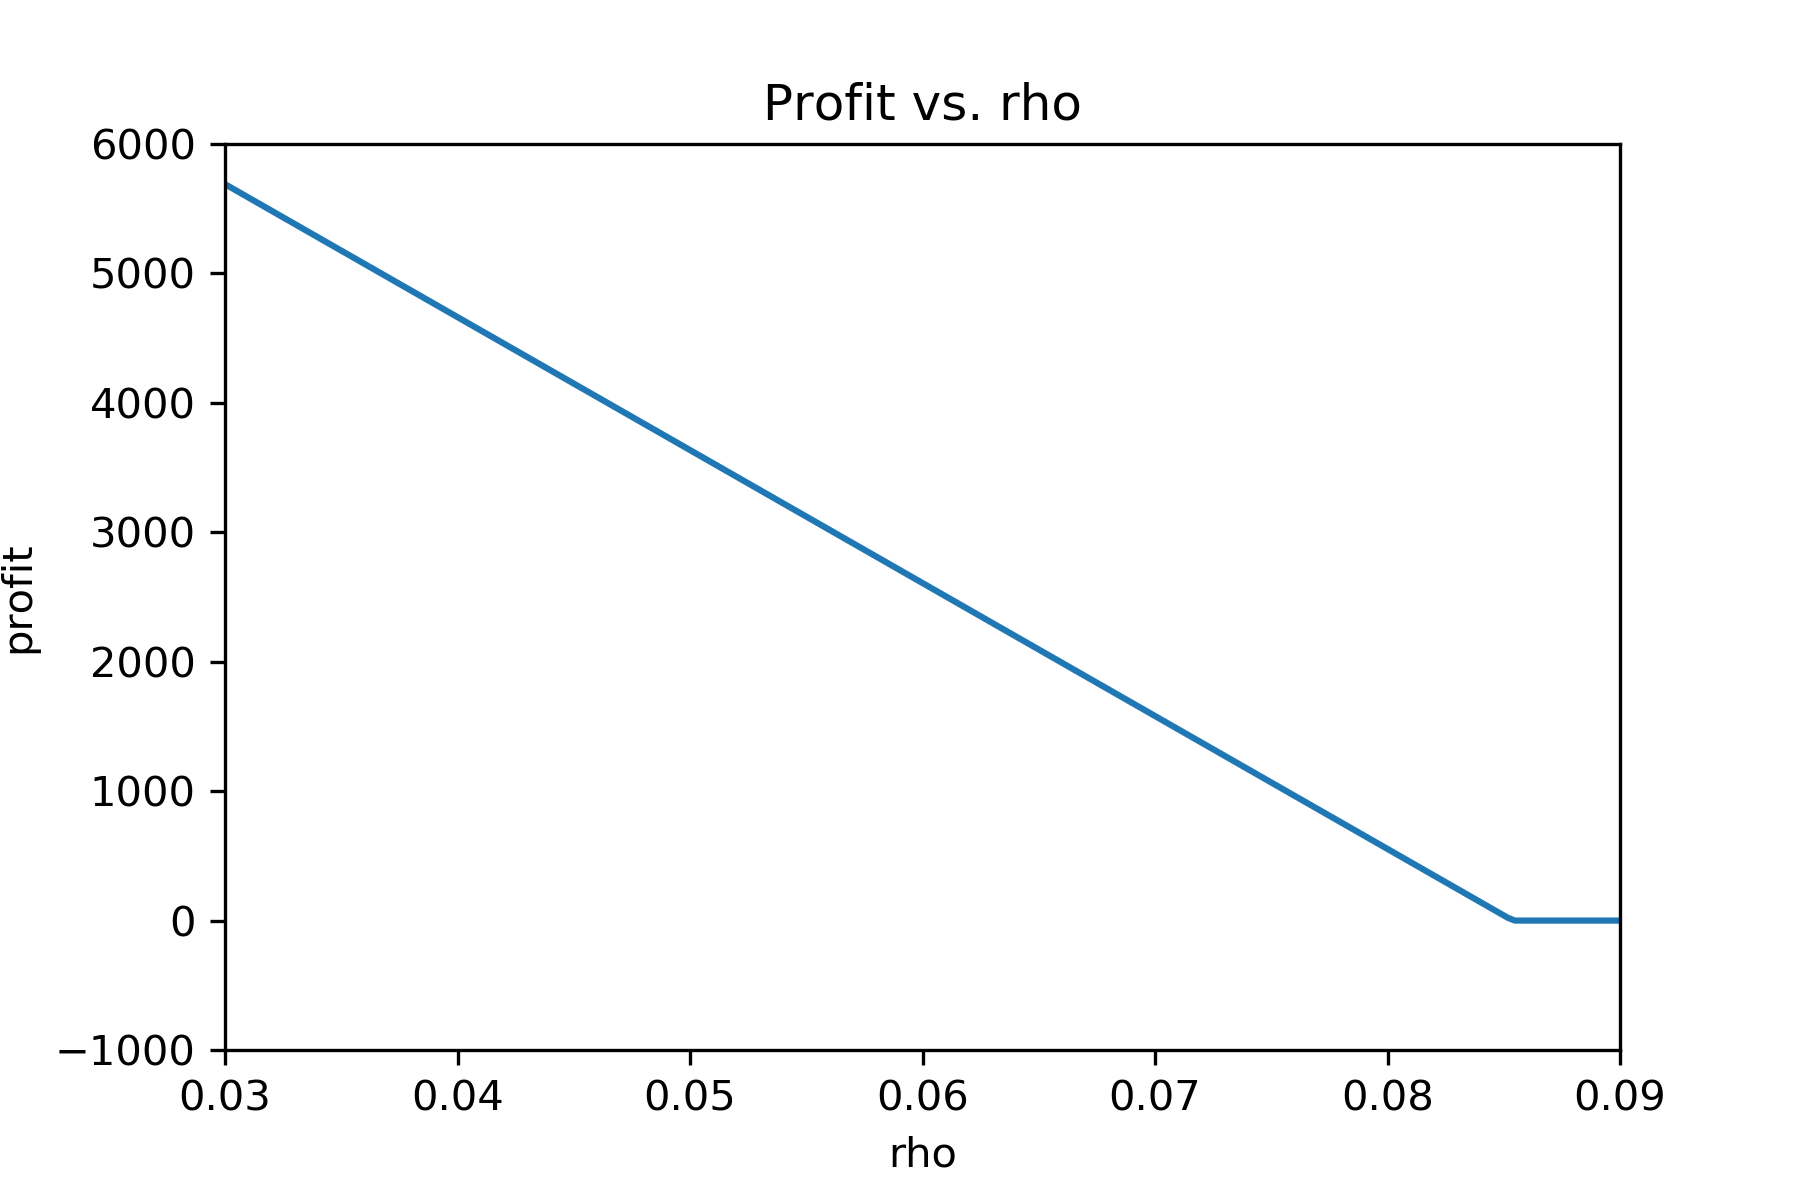
\includegraphics[width=0.5\textwidth]{problem5_profit_vs_rho.png}}
    \end{figure}
\end{enumerate}
\end{solution}

\newpage
\subsection*{Exercise 6 (Robust linear programming)}

In this problem we will consider a version of linear programming under uncertainty.
\begin{enumerate}
    \item Let $x \in \mathbb{R}^n$ be a given vector. Prove that $x^Ty \leq \|x\|_1$ for all $y$ such that $||y||_{\infty} \leq 1$. Is this inequality tight? (Is there always a $y$ such that the equality holds ?)
\end{enumerate}

Let us focus now on a LP in standard form:
\begin{align}
    &\min_x c^Tx \nonumber \\
    \label{LP}
    \text{s.t.} \; \; &a_i^Tx \leq b_i, \; \; i = 1,...,m
\end{align}

Consider the set of linear inequalities in (\ref{LP}). Suppose you don't know the coefficients $a_i$ exactly. Instead you are given nominal values $\overline{a}_i$, and you know that the actual coefficient vectors satisfy $\|a_i - \overline{a}_i\|_{\infty} \leq \rho $ for a given $\rho > 0$. In other words, the actual coefficients $a_{ij}$ can be anywhere in the intervals $[\overline{a}_{ij} - \rho, \overline{a}_{ij} + \rho]$.  or equivalently, each vector $a_i$ can lie anywhere in a rectangle with corners $\overline{a}_i + v$ where $v \in \{-\rho, \rho\}^n$. The set of inequalities that constrain problem~\ref{LP} must be satisfied for all possible values of $a_i$; i.e., we replace these with the constraints
    \begin{equation}
    \label{rob_constr}
           a_i^Tx \leq b_i \; \; \forall a_i \in \{\overline{a}_i + v \; \mid \|v\|_{\infty} \leq \rho \} \; \;  i = 1, ..., m.
    \end{equation}

    A straightforward but very inefficient way to express this constraint is to enumerate the $2^n$ corners of the rectangle of possible values $a_i$ and to require that
    \[
    \overline{a}_i^Tx + v^Tx \leq b_i \; \; \forall v \in \{-\rho, \rho\}^n \; \; i = 1, ..., m.
    \]

    \begin{enumerate}
    \item[2.]
    Use the previous result to show that (\ref{rob_constr}) is in fact equivalent to the much more compact set of nonlinear inequalities
    \[
        \overline{a}_i^Tx + \rho\|x\|_1 \leq b_i, \; \; i = 1,...,m.
    \]

    \end{enumerate}

    We now would like to formulate the uncertainty in the LP we introduced. We are therefore interested in situations where the coefficient vectors $a_i$ are uncertain, but satisfy bounds $\|a_i - \overline{a}_i\|_{\infty} \leq \rho$  for given $\overline{a}_i$ and $\rho$. We want to minimize $c^Tx$ subject to the constraint that the inequalities $a_i^Tx \leq b_i$ are satisfied for $\textit{all}$ possible values of $a_i$. \\ \\
    We call this a $\textit{robust LP}:$
    \begin{align}
    &\min_x c^Tx \nonumber \\
    \label{RLP}
    \text{s.t.} \; \;  &a_i^Tx \leq b_i, \; \; \forall a_i \in \{ \overline{a}_i + v \mid \|v\|_{\infty} \leq \rho \} \; \; \; i = 1,...,m.
\end{align}

\begin{enumerate}
    \item[3.] Using the result from part 2, express the above optimization problem as an LP.

\end{enumerate}

\begin{solution}
% Your solution here
\end{solution}

\end{document}
